\subsection{BitVM2}

We will outline the overall design and then address some challenges that require future resolution and optimization.

\subsubsection{Overall Design}

The overall design of BitVM2 within Fiamma is as follows:

\begin{figure}[ht] 
    \centering  
    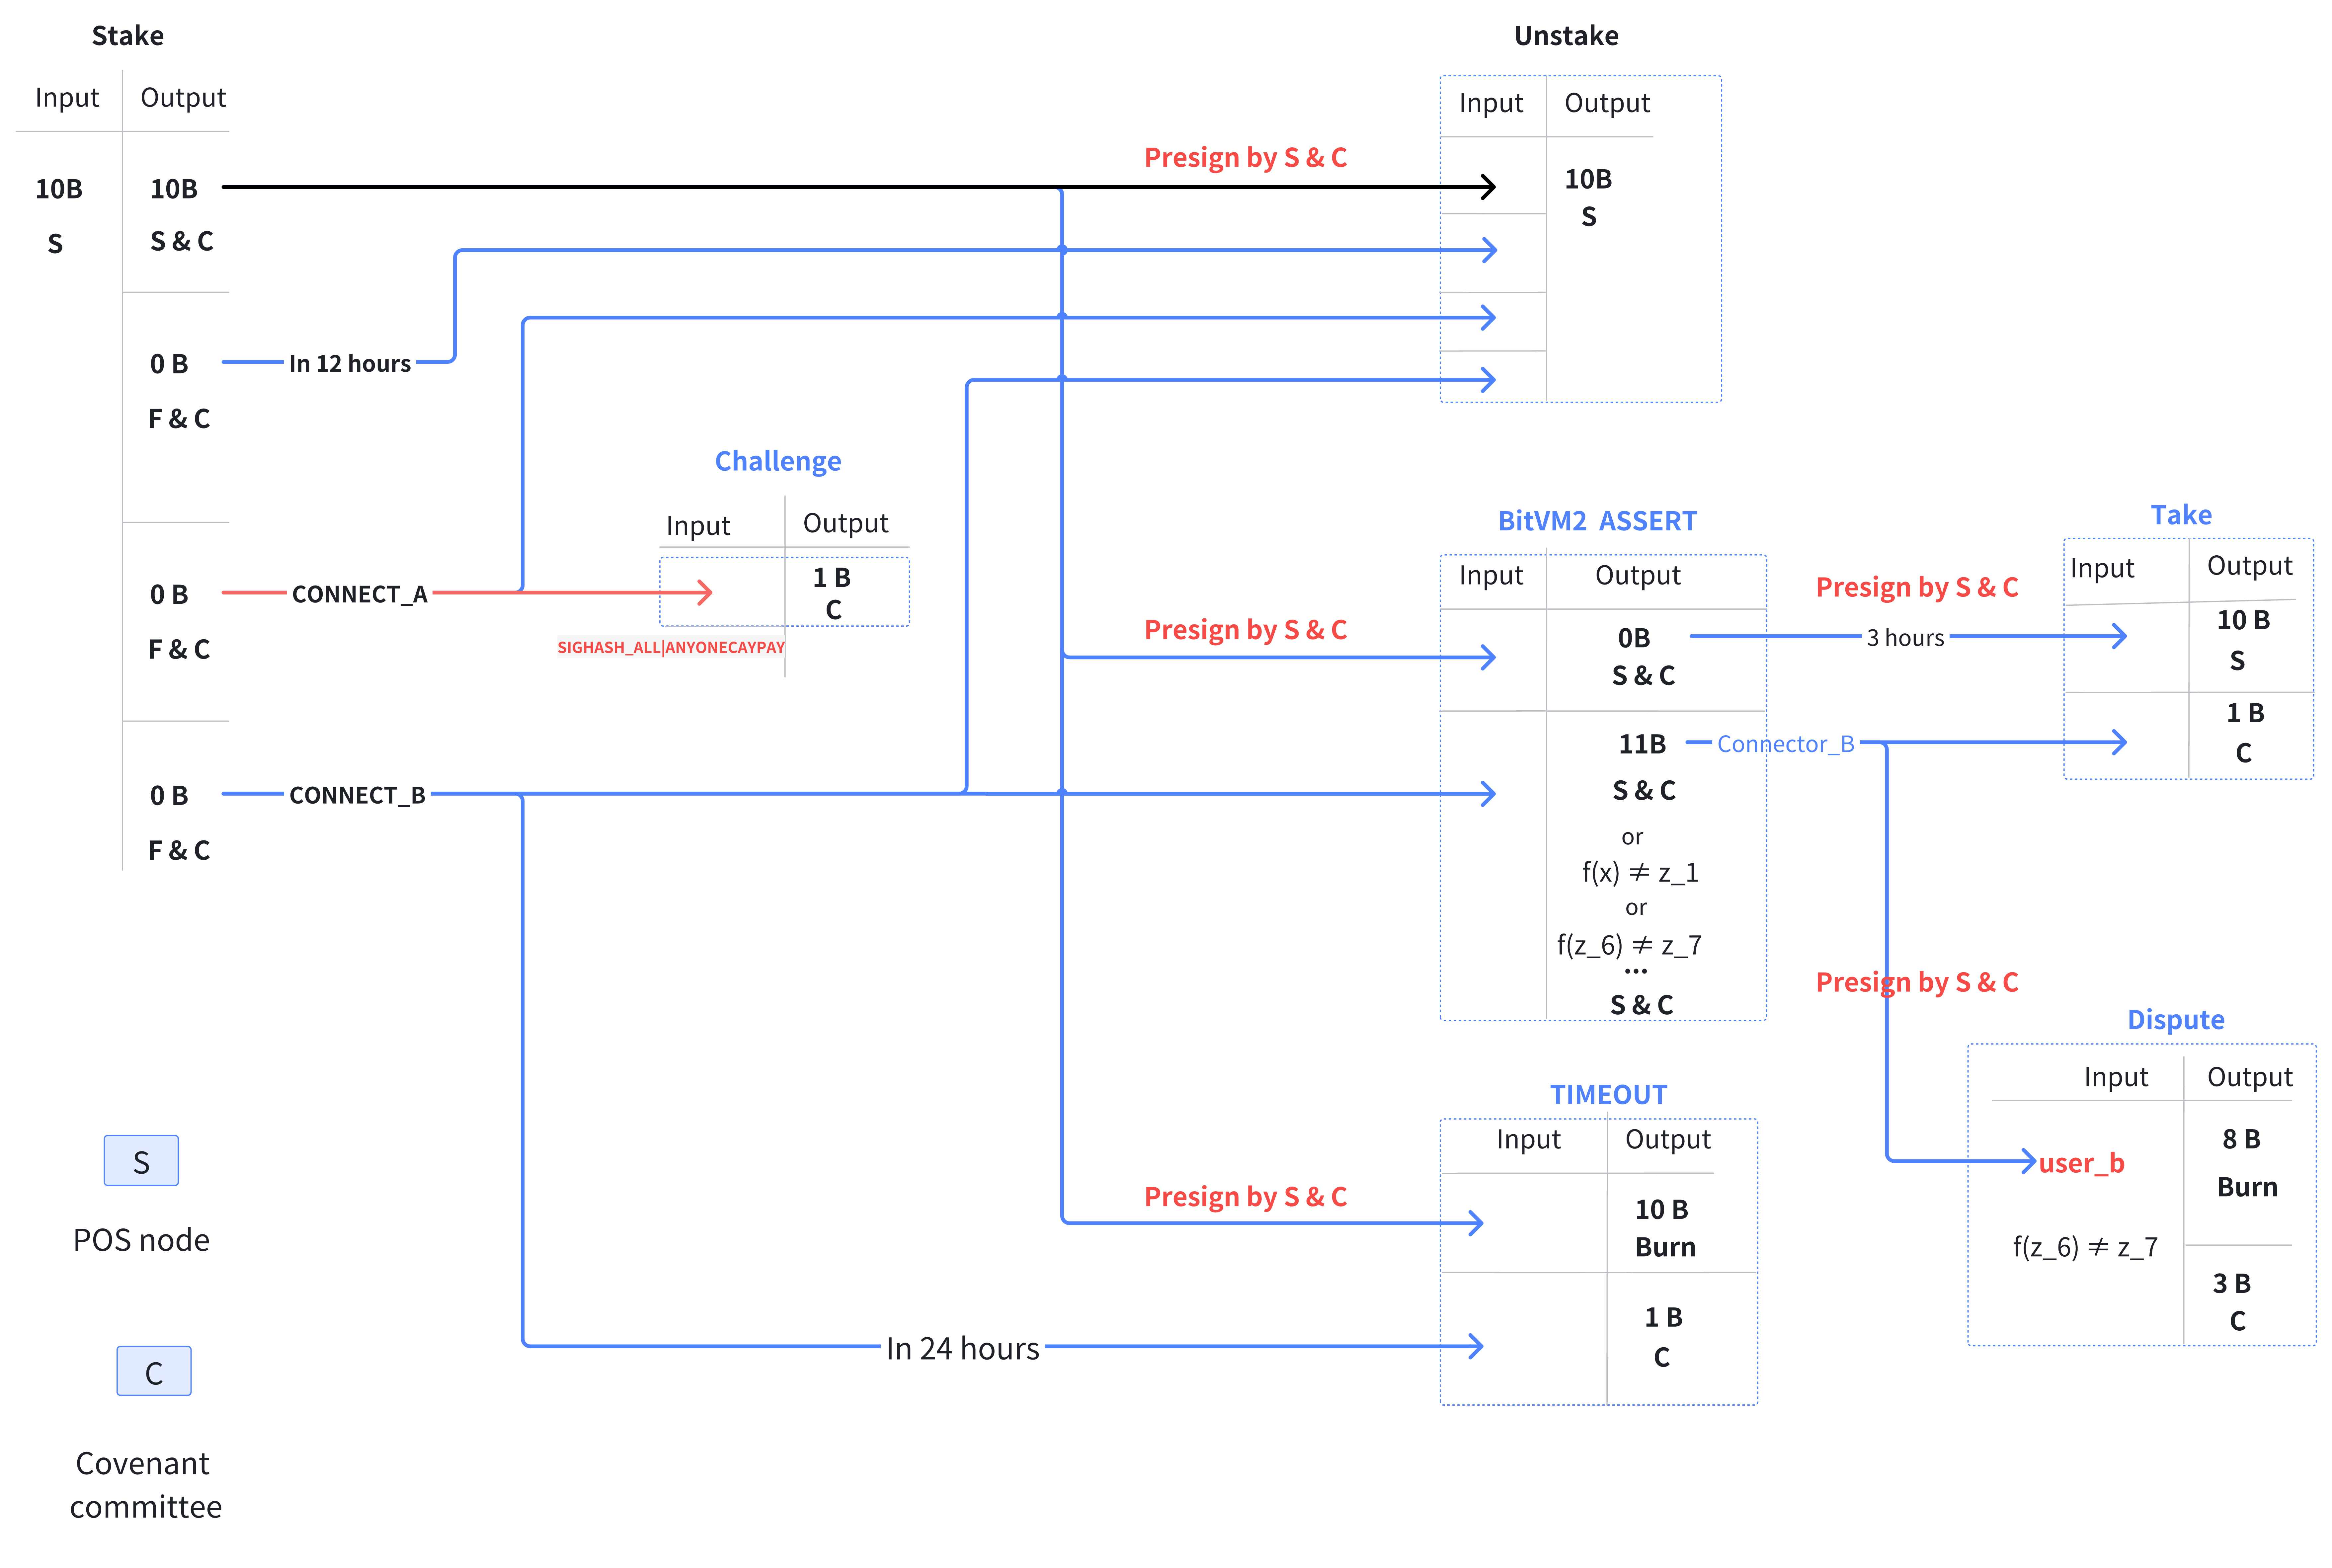
\includegraphics[width=0.85\columnwidth]{images/bitvm2 protocol.png} 
    \caption{bitvm2 protocol}
    \label{fig:bitvm2 protocol}
\end{figure}

Now, we will further explain the design in 3 paragraphs

\paragraph{Roles}

We will introduce the roles first:

\begin{itemize}
    \item \textbf{S}: The staker, the individual who stakes BTC to become a PoS node in Fiamma.
    \item \textbf{C}: The Committee, made up of important partners of Fiamma.
    \item \textbf{Challenger}: The individual who is willing to kick off the challenge by paying 1 BTC.
    \item \textbf{user\_b}: The individual who kicks off the dispute transaction on Bitcoin.
\end{itemize}

\paragraph{Transactions}

We introduce the function of each transaction:

\begin{itemize}
    \item \textbf{Stake transaction}: Somebody stakes, e.g., 5 BTC, as a PoS node of Fiamma by issuing a Stake transaction.
    \item \textbf{Unstake transaction}: S can take back the staking asset at any time by issuing an Unstake transaction.
    \item \textbf{Challenge transaction}: Challenger could kick off the Challenge transaction by paying 1 BTC. It should be noted that it is permissionless to become a Challenger.
    \item \textbf{Assert transaction}: Generate a taproot address and then transfer the staked BTC to the taproot address. Anyone could spend this taproot address if he can provide a valid witness of any leaf.
    \item \textbf{Take transaction}: Return the staked BTC to S if no one can spend from the Taproot address within a specified time period; the Challenger forfeits 1 BTC.
    \item \textbf{Dispute transaction}: Anyone can initiate this transaction if they are able to spend from the Taproot address; S will be slashed as a result.
    \item \textbf{Timeout transaction}: If a challenge occurs, S can still be slashed if the Assert transaction is not initiated within a specified time frame.
\end{itemize}


\paragraph{Overall flow}

We will present the overall flow of the entire protocol in the following diagram:

\begin{figure}[ht] 
    \centering  
    \includegraphics[width=0.85\columnwidth]{images/bitvm2 simple flow.png} 
    \caption{Simplified flow of the protocol}
    \label{fig:bitvm2 simple flow}
\end{figure}

\begin{itemize}
    \item S stakes, for example, 5 BTC, to become a PoS node in Fiamma.
    \item Initially, S pre-signs six transactions with the Committee (services will be withheld if S fails to sign these transactions).
    \item S provides ZKP verification services on the Fiamma chain and stores inputs, outputs, and all intermediate values on the PoS chain, along with the Winternitz signature for these values.
    \item At this phase, the proof state reaches soft finality, indicating it is secured by the PoS network up to this point.
    \item Intersubjective nodes in Fiamma actively monitor the PoS chain and access proofs in soft finality.
    \item When the proof receives enough confirmations, exceeding a pre-defined threshold, its state transitions to hard finality.
    \item If any single intersubjective node is honest, it can detect a false claim by S and initiate the Challenge transaction.
    \item S broadcast the Assert transaction
    \item Anyone (usually user\_b, who is often the Challenger) initiates the Dispute transaction.
    \item Subsequently, S is slashed.
    \item If the Dispute transaction is not initiated within a specified timeframe, S reclaims the assets by issuing the Take transaction.
\end{itemize}

\subsubsection{Core features}

Our protocol exhibits several key properties as follows:

\begin{itemize}
    \item \textbf{Trustless Asset Security}: The assets are secure without introducing any additional assumptions.
    \item \textbf{Trust-Minimized Protocol}: If S is malicious, they will be slashed if any single intersubjective node is honest.
    \item \textbf{Decentralized Network}: Intersubjective nodes are permissionless, ensuring the protocol is both decentralized and secure.
    \item \textbf{Economic Incentives}: S and intersubjective nodes are deterred from malicious actions by punitive mechanisms. Nodes are incentivized to challenge if S is malicious, due to the potential rewards.
\end{itemize}


\subsubsection{To be Improved and Completed}

The protocol described previously represents an ideal case; however, several aspects still require attention, improvements, and completion:

\begin{itemize}
    \item \textbf{BTC Slashing}: Currently, Babylon supports only double-sign faults, necessitating that PoS nodes stake additional BTC to cover validity faults. Improvements will follow once Fiamma assists Babylon in integrating the BitVM2 component.
    \item \textbf{Reward Delivery}: It is not possible to identify the Challenger in advance during the initial phase; therefore, the Committee will handle this aspect.
    \item \textbf{Security}: The protocol is secure provided that neither S nor C act maliciously at the same time.
    \item \textbf{Staking for Intersubjective Nodes}: Intersubjective nodes are required to stake assets on Fiamma or Bitcoin to prevent outages or malicious behavior.
    \item \textbf{On-chain Cost for Challenge Process}: Since there is no need to store data and commitments on Bitcoin, efforts should continue to minimize the size of all subscripts to reduce challenge costs.
    \item \textbf{Blake3 Hash Integration}: We are actively integrating the Blake3 hash into the Winternitz signature system \cite{website:witernitz}.
    \item \textbf{Winternitz Signature}: We will complete the integration of the Winternitz signature in the next phase.
\end{itemize}
